%%%%%%%%%%%%%%%%%%%%%%%%%%%%%%%%%%%%%%%%%
% Short Sectioned Assignment LaTeX Template Version 1.0 (5/5/12)
% This template has been downloaded from: http://www.LaTeXTemplates.com
% Original author:  Frits Wenneker (http://www.howtotex.com)
% License: CC BY-NC-SA 3.0 (http://creativecommons.org/licenses/by-nc-sa/3.0/)
%%%%%%%%%%%%%%%%%%%%%%%%%%%%%%%%%%%%%%%%%

%----------------------------------------------------------------------------------------
%	PACKAGES AND OTHER DOCUMENT CONFIGURATIONS
%----------------------------------------------------------------------------------------

\documentclass[paper=a4, fontsize=11pt]{scrartcl} % A4 paper and 11pt font size

% ---- Entrada y salida de texto -----

\usepackage[T1]{fontenc} % Use 8-bit encoding that has 256 glyphs
\usepackage[utf8]{inputenc}
%\usepackage{fourier} % Use the Adobe Utopia font for the document - comment this line to return to the LaTeX default

% ---- Idioma --------

\usepackage[spanish, es-tabla]{babel} % Selecciona el español para palabras introducidas automáticamente, p.ej. "septiembre" en la fecha y especifica que se use la palabra Tabla en vez de Cuadro

% ---- Otros paquetes ----

%https://en.wikibooks.org/wiki/LaTeX/Hyperlinks#.5Curl
\usepackage[colorlinks=true,linkcolor=blue,citecolor=red, urlcolor=blue]{hyperref} % para poder poner referencias, url...

%https://en.wikibooks.org/wiki/LaTeX/Colors
\usepackage{color, colortbl}
\usepackage[first=0,last=9]{lcg} %Color tabla
\newcommand{\ra}{\rand0.\arabic{rand}} %Color tabla

\usepackage{eurosym} %Símbolo del euro

\usepackage{amsmath,amsfonts,amsthm} % Math packages
%\usepackage{graphics,graphicx, floatrow} %para incluir imágenes y notas en las imágenes
\usepackage{graphics,graphicx, float, url} %para incluir imágenes y colocarlas

% Para hacer tablas comlejas
%\usepackage{multirow}
%\usepackage{threeparttable}

%\usepackage{sectsty} % Allows customizing section commands
%\allsectionsfont{\centering \normalfont\scshape} % Make all sections centered, the default font and small caps

\usepackage{fancyhdr} % Custom headers and footers
\pagestyle{fancyplain} % Makes all pages in the document conform to the custom headers and footers
\fancyhead{} % No page header - if you want one, create it in the same way as the footers below
\fancyfoot[L]{} % Empty left footer
\fancyfoot[C]{} % Empty center footer
\fancyfoot[R]{\thepage} % Page numbering for right footer
\renewcommand{\headrulewidth}{0pt} % Remove header underlines
\renewcommand{\footrulewidth}{0pt} % Remove footer underlines
\setlength{\headheight}{13.6pt} % Customize the height of the header

\numberwithin{equation}{section} % Number equations within sections (i.e. 1.1, 1.2, 2.1, 2.2 instead of 1, 2, 3, 4)
\numberwithin{figure}{section} % Number figures within sections (i.e. 1.1, 1.2, 2.1, 2.2 instead of 1, 2, 3, 4)
\numberwithin{table}{section} % Number tables within sections (i.e. 1.1, 1.2, 2.1, 2.2 instead of 1, 2, 3, 4)

\setlength\parindent{0pt} % Removes all indentation from paragraphs - comment this line for an assignment with lots of text

\newcommand{\horrule}[1]{\rule{\linewidth}{#1}} % Create horizontal rule command with 1 argument of height

\usepackage{enumerate}
\usepackage{listings}
\usepackage{amsmath}%
\usepackage{amsfonts}%
\usepackage{amssymb}%
\usepackage{MnSymbol}%
\usepackage{wasysym}%
\usepackage{graphicx}
\usepackage{grffile}
\usepackage[spanish]{babel}
\usepackage{babel}
\usepackage{tikz}
\usetikzlibrary{babel}
\usepackage{color}
\usepackage{hyperref}
\usepackage{setspace}

\definecolor{dkgreen}{rgb}{0,0.6,0}
\definecolor{gray}{rgb}{0.5,0.5,0.5}
\definecolor{mauve}{rgb}{0.58,0,0.82}
\definecolor{LightCyan}{rgb}{0.88,1,1}

\lstset{frame=tb,
	language=Java,
	aboveskip=3mm,
	belowskip=3mm,
	showstringspaces=false,
	columns=flexible,
	basicstyle={\small\ttfamily},
	numbers=none,
	numberstyle=\tiny\color{gray},
	keywordstyle=\color{blue},
	commentstyle=\color{dkgreen},
	stringstyle=\color{mauve},
	breaklines=true,
	breakatwhitespace=true,
	tabsize=3
}

%----------------------------------------------------------------------------------------
%	TÍTULO Y DATOS DEL ALUMNO
%----------------------------------------------------------------------------------------

\title{
\normalfont \normalsize
\textsc{ Programación de Dispositivos Móviles (2017-2018)\\
			Grado en Ingeniería Informática\\ 
			Universidad de Granada}
			\\ [25pt] % Your university, school and/or department name(s)
\horrule{0.5pt} \\[0.4cm] % Thin top horizontal rule
\huge Tutorial 1\\ % The assignment title
\horrule{2pt} \\[0.5cm] % Thick bottom horizontal rule
}

\author{ Juan Alberto Martínez López \\ Alberto Armijo Ruiz \\}

\date{\normalsize\today} % Incluye la fecha actual



%----------------------------------------------------------------------------------------
% DOCUMENTO
%----------------------------------------------------------------------------------------

\begin{document}

\maketitle % Muestra el Título


\includegraphics[width=1\linewidth]{ugr}

\newpage %inserta un salto de página

\tableofcontents % para generar el índice de contenidos

%\listoffigures

%\listoftables

\newpage

%----------------------------------------------------------------------------------------
%	Introducción
%----------------------------------------------------------------------------------------

\section{Introducción}

Para esta práctica hemos desarrollado el algoritmo Miller-Rabin para decidir si un número es posible primo o no es primo, para ello hemos desarrollado dos versiones del algoritmo: Una en la que se realizan n aplicaciones para comprobar la primalidad y otro con una lista de números naturales con los que se comprueba el test para el primo y cada una de las bases de la lista. Para calcular la primalidad utilizamos el algoritmo de logaritmo discreto en el que comprobamos la existencia dado a,b y p de $\log_a (b) \mod n$ y si se cumple el número es primo.

\section{Evaluación de tiempos}

Para el algoritmo Miller-Rabin con 2000 aplicaciones podemos apreciar muy poco aumento del tiempo (Tabla 1.1), por lo que podemos concluir que el procesamiento de la primalidad no tiene una carga grande y no hay problema a la hora de calcular números grandes.
\begin{table}[htbp]
	\begin{center}
		\begin{tabular}{|l|l|}
			\hline
			\rowcolor{LightCyan}
			Número Primo & Tiempo ejecución (seg) \\ \hline
			57347&  0.008280 \\ \hline 
			468577&  0.009140 \\ \hline 
			5555567&  0.013386 \\ \hline 
			87654337&  0.012030 \\ \hline 
			987654323&  0.014271 \\ \hline 
			3141592661&  0.019104 \\ \hline 
			11111111113&  0.020818 \\ \hline 
			121212121223&  0.021233 \\ \hline 
			2718281828489&  0.025449 \\ \hline 
			16180339892149&  0.027566 \\ \hline 
			800000000000017&  0.031171 \\ \hline 
		\end{tabular}
		\caption{Tabla tiempos de ejecución para el algoritmo Miller Rabin}
		\label{tabla:millerrabin}
	\end{center}
\end{table}

\begin{figure}[H]
	\begin{center}
		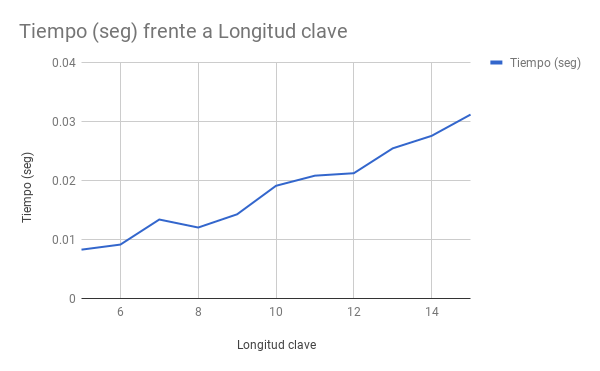
\includegraphics[width=1\linewidth]{chart2}
		\caption{Tiempos vs Longitud clave Miller-Rabin}
		\label{figura: tiempos3}
	\end{center}
\end{figure}

Como se puede ver en la gráfica y en la tabla, los tiempos de ejecución son pequeños, y sigue una distribución lineal dependiendo del tamaño del número primo. 

Para el algoritmo del logaritmo discreto se han calculado una a y c aleatoria y hemos calculado la b a partir de $b = a^c\mod p$. En las tablas 1.2 y 1.3 si que se puede apreciar un aumento considerable de los tiempos ya que de un tiempo a otro podemos ver como se cuadruplican de un resultado a otro. \\

\begin{table}[htbp]
	\begin{center}
		\begin{tabular}{|l|l|}
			\hline
			\rowcolor{LightCyan}
			Longitud clave & Tiempo ejecución (seg) \\ \hline
			5 & 0.001187 \\ \hline 
			6 & 0.004052 \\ \hline
			7 & 0.018117 \\ \hline
			8 & 0.080128\\ \hline
			9 & 0.289543\\ \hline
			10 & 0.73591\\ \hline
			11 & 1.506318\\ \hline
			12 & 5.264323\\ \hline
			13 & 29.752512\\ \hline
			14 & 76.744032 \\ \hline
			15 & 612.546521\\ \hline
		\end{tabular}
		\caption{Tabla tiempos}
		\label{tabla:resumen}
	\end{center}
\end{table}


\begin{table}[htbp]
	\begin{center}
		\begin{tabular}{|l|l|l|l|l|}
			\hline 
			\rowcolor{LightCyan}
			A & B & P & Solución & Tiempos (s) \\ \hline
			6 & 50628 & 57347& 7 & 0.001187 \\ \hline 
			8 & 449605 & 468577& 11 & 0.004052 \\ \hline
			207 & 4374842 & 5555567& 104 & 0.018117 \\ \hline
			4007 & 8515459 & 87654337& 430 & 0.080128\\ \hline
			40756 & 118205788 & 987654323& 10748 & 0.289543\\ \hline
			20544 & 253647140 & 3141592661& 113 & 0.735911\\ \hline
			112354 & 9048018943 & 11111111113& 5658 & 1.506318\\ \hline
			1245628 & 49579028347 & 121212121223& 568985 & 5.264323\\ \hline
			87569 & 1342094524016 & 2718281828489& 5749833 & 29.752512\\ \hline
			568236 & 14717101287551 & 16180339892149& 389567512 & 76.744032\\ \hline
			4555786 & 778596955901441 & 800000000000017& 785951 & 612.546521\\ \hline
		\end{tabular}
		\caption{Tabla análisis de logaritmo.}
		\label{tabla:compleja}
	\end{center}
\end{table}

En la siguiente figura podemos apreciar como el crecimiento del tiempo de ejecución tiene forma de una función exponencial.\\

\begin{figure}[H]
	\begin{center}
		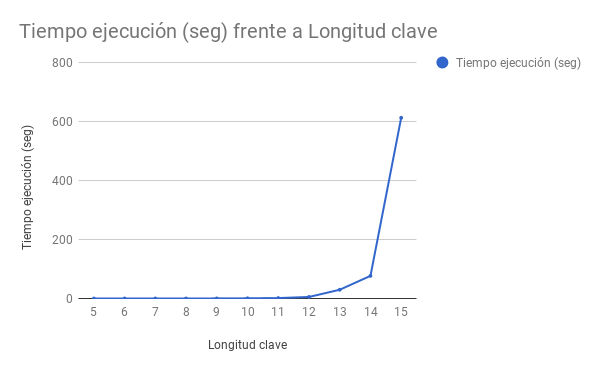
\includegraphics[width=1\linewidth]{chart}
		\caption{Tiempos vs Longitud clave}
		\label{figura: tiempos}
	\end{center}
\end{figure}

Si le metemos una escala logarítmica vemos como la función es casi lineal.
\begin{figure}[H]
	\begin{center}
		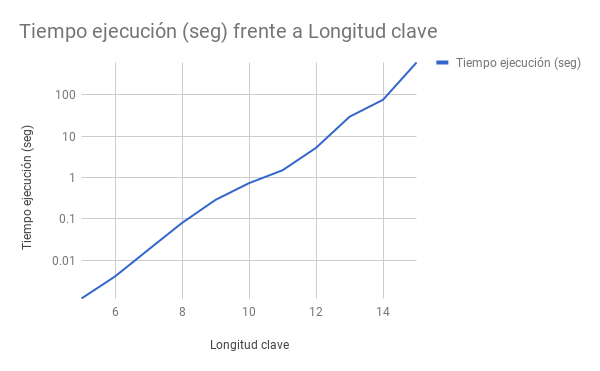
\includegraphics[width=1\linewidth]{chart1}
		\caption{Tiempos vs Longitud clave escala logaritmica}
		\label{figura: tiempos2}
	\end{center}
\end{figure}



Hemos calculado la media armónica entre un tiempo y el siguiente es de 3.47 el cual podemos aproximarlo a 4. De manera que dado un tamaño de X cifras, el tiempo aproximado de ejecución sería de $4^X$ por lo que para números grandes el tiempo necesario de ejecución sería enorme.\\

El algoritmo además ocupa una gran cantidad de RAM, ya que para la clave de mayor tamaño ha llegado a ocupar 4.2 Gb.\\

\section{Conclusión}

Sobre el algoritmo Miller-Rabin podemos concluir que es un algoritmo eficiente para calcular si un número es primo, aunque debemos tener en cuenta que la solución que nos da no es exacta en caso positivo, es decir cuando puede que sea primo. \\

El algoritmo que resuelve el problema del logaritmo discreto (algoritmo Big step, baby step) no tiene una gran eficiencia a la hora de procesar números grandes ya que si por ejemplo ejecutamos el algoritmo con una clave de 50 cifras tendríamos que $4^(50) = 4.02 e+19$ años, lo que sería demasiado tiempo para descodificar una clave de ese tamaño.\\

\section{Instrucciones para su ejecución en Linux}
Para poder ejecutar el código en Linux es necesario tener instalado antes python3. Si lo tenemos instalado deberemos hacer lo siguiente:\\
\begin{enumerate}
	\item Descargar el directorio que contiene el archivo ejecutable. Llamado Practica1\_AA\_JA.zip
	\item Descomprimir el contenido de la carpeta.
	\item Acceder a la carpeta que hemos descomprimido. Para ello hay que utilizar el comando cd Practica1 desde el directorio en el que se haya descomprimido.
	\item Para ejecutar el archivo main.py hay que ejecutar el siguiente comando:
	\begin{lstlisting}
		python3 main.py <nombre_del_archivo_de_pruebas>
	\end{lstlisting}
\end{enumerate}

\end{document}